\documentclass[a4paper]{scrartcl}

\newif\ifhtml

% HTML generation (.doc-conversion) > set html to true and use htlatex. else set html to false
%\htmltrue
\htmlfalse

\ifhtml % In case of web format output...
	\def\pgfsysdriver{pgfsys-tex4ht.def}
	\usepackage[dvips]{graphicx}
\else
	\usepackage[pdftex]{graphicx}
\fi

\usepackage[ansinew]{inputenc}	% so I can write my Name without \"{u}
\usepackage[T1]{fontenc}        % Standard Latex-Fonts
\usepackage[english]{babel}     % change [english] if written in other language
\usepackage{svn-multi}          % to add SVN-Versioning-Info
\usepackage{subfig}             % subfigures
\usepackage[Gray]{SIunits}      % typographically correct units (\milli\meter, \kilo\electronvolt)
\usepackage{booktabs}           % nice tables
\usepackage{fancyhdr}           % nice header
\usepackage{tikz}				% extremely nice drawings
\usepackage{microtype}          % for nicer typography
\usepackage[numbers,square,sort&compress]{natbib} % nice bibliography
%\usepackage{flafter}           % floats after their first instance
%\usepackage{setspace}
%	\doublespacing
%	\onehalfspacing
%	\singlespacing

\ifhtml
	\usepackage{index}
	\usepackage{color}
	\newindex{todo}{todo}{tnd}{Todo List} 
	\newcommand{\todo}[1]{\textcolor{red}{[To do: #1]}\index[todo]{#1}}
	\usepackage{url}
\else
	\usepackage{lmodern}
	\usepackage{lineno}
	% line numbers
	\linenumbers
	%%\pagewiselinenumbers
	\modulolinenumbers[2]
	\usepackage[backref,pdftex]{hyperref}			% backref generates link from references back to text
	\usepackage{todonotes}
	\hypersetup{colorlinks=false,%
			pdfauthor={David Haberth�r},%
			pdftitle={Progress Report for the Graduate School for Cellular and Biomedical Sciences - 2008},%
			pdfsubject={Progress Report},%
			pdfkeywords={skeletonization, tomography, biomedical imaging, SRXTM},%
			pdfborder={0 0 0},% > no border around links, needs the line below to really make sense
			colorlinks=true % colored links instead of colorfully framed links.
			}
\fi

%% Subversion Information
\svnidlong
{$HeadURL$}
{$LastChangedDate$}
{$LastChangedRevision$}
{$LastChangedBy$}
\svnid{$Id$}

\pagestyle{fancy}
%%%
\cfoot{}
\rfoot{}
%%%
%\fancyhead{}
%\fancyfoot{}
%\fancyhead[RO]{{\footnotesize\rightmark}}
%\fancyfoot[RO]{\thepage}
%\fancyhead[LE]{{\footnotesize\leftmark}}
%\fancyfoot[LE]{\thepage}
%%svn-info in footer, page in header
\fancyfoot[C]{\tiny{URL: \url{\svnkw{HeadURL}} ; \space Last changed on: \svnkw{LastChangedDate} ; \space Revision: \svnkw{LastChangedRevision} ; \space Author: \svnkw{LastChangedBy}}}
%\fancyfoot[RO]{\tiny{URL: \url{\svnkw{HeadURL}} ; \space Last changed on: \svndate ; \space Revision: \svnrev ; \space Author: \svnFullAuthor*{\svnauthor}}}
%\fancyhead[C]{page \thepage}
%%svn-info in footer, page in header
%\renewcommand{\headrulewidth}{0.3pt}

\newcommand{\imsize}{\linewidth}

\title{Progress Report for the Graduate School for Cellular and Biomedical Sciences - 2008}
\author{David Haberth�r}
\date{Version of \today}

\begin{document}
\maketitle

\ifhtml
	\emph{Did you sort out all to dos?}
\else
	\listoftodos
\fi

%\tableofcontents

\section{Introduction}
Analogous to to the last submitted progress report from February 19, 2008, I have focused on different tasks during the past year. The basis of my work is the data obtained with synchrotron radiation based x-ray tomographic imaging (SRXTM) at the TOMCAT beamline~\cite{Stampanoni2007} of the Swiss Light Source (SLS) at the Paul Scherrer Institut (PSI) in Villigen, Switzerland.

The past year I have focused on multimodal imaging to detect sub-micron particles in the lung and on the  skeletonization of the terminal airways. As I have stated in the last progress report, the multimodal imaging approach I was working on has been overcome by recent progressions at TOMCAT and is now no longer followed actively in our group. Nevertheless we were able to match results from two imaging modalities; the results obtained with this method and the nanoparticle detection and assessment of the agreement between conventional electron microscopy and SRXTM has been presented as a poster at three meetings and submitted as a proceeding to the journal of physics (see section~\ref{sec:publications}).

During the past summer months I had the possibility to conduct the thesis of my Master of Advanced Studies ETH in Medical Physics directly involved with the development of a new scanning protocol at the TOMCAT beamline, working for two full months at the PSI, while being integrated in the group we otherwise closely collaborate. The details of this newly developed method are described in section~\ref{sec:wide field scanning}. The developed method is planned to be implemented for end-user access at the beamline early next year.

\section{SRXTM}
During three regularly allotted beam times we obtained tomographic datasets of 67 samples while performing 151 scans in total. The difference between the amount of samples arises through the use of a novel imaging method, which uses multiple partial scans to obtain tomographic images of one sample and is described later on. During the term of my master thesis I additionally perform 17 scans during the so called ``in house development'' time at the beamline to proof the simulated predictions made during the development of the wide field scanning method.

Most of the samples we recorded, were obtained from lung samples from R108-rats\todo{details and citation needed!}. During the third beamtime in 2008 we also obtained tomographic scans of mice bones \todo{citation needed, explain the details of this experiment} (tibia, femur and vertebrae) to asses the trabecular structure of these bones. This particular experiment has been performed as part of a collaboration with the University of G�ttingen, Germany. 

%08a - 42 samples, 1 ruler
%08b - 10 samples: wide field scanning (38 scans (4*5, 6*3))
%08c - 15 samples: 1 normal, 13*360, 19*wfs a je 3 subscans 
% masterarbeit 17* R108C60_22_20x
                              
All my projects involve SRXTM to a certain degree, generally as a basis for image or data acquisition. The three following sections of this progress report discuss three of my major projects for the past year.

\section{Multimodal Imaging}
\label{sec:multimodal imaging}
Even if my intentions to build up a multimodal toolchain for the imaging of lung samples has been caught up by developments at the beamline, we still have been very successful with the direct comparison of conventional transmission electron microscopy images (TEM, with a resolution around \unit{1}{\nano\meter}) and slices from our three dimensional dataset obtained with SRXTM (with a resolution of \unit{350}{\nano\meter}). We applied sub-micron sized gold particles to rat lungs and obtained tomographic scans of these lung samples at TOMCAT.

With conventional TEM imaging we cannot obtain unrestricted three dimensional information from the scanned samples, mostly because the sample has to be cut into serial sections. With carefully controlled experimentation methods we have been able to match real TEM slices with virtual slices from the SRXTM dataset. This enabled us to use the ultrahigh resolution TEM images for the the characterization of sub-micron particles in the mammalian lung and to localize these single and clustered gold particles in alveoli, alveolar ducts and small bronchioli using the fully unrestricted three dimensional dataset obtained with SRXTM.

We have been able to show the excellent agreement between those two imaging modalities and have submitted theres results to the Journal of Physics (see~\cite{Haberthuer2009}, of which a copy is attached to this document).

\section{Skeletonization}
\label{sec:skeletonization}
During the last weeks of 2007 I have started to develop a method for the extraction of structural information from the scanned lung samples. The method has been refined to such a degree that I have been able to extract the first partial acinar airway skeleton of a mammalian lung that has ever been extracted. There have been publications on the extraction of an airway skeleton before~\cite{Hasegawa2006,Sauret1999,Suter2004}, but none of the airway skeletons ever published is on such a minute level as we are now able to provide it. \citet{Sauret1999} state, that the slice thickness of their computed tomography images is \unit{1}{\milli\meter}, while the dimensions our whole sample is around \unit{2}{\milli\meter}, so we roughly have a resolution that is about 1000 $\times$ finer than what has been achieved up to now.

\subsection{Method}
I have been using the free Medical Image Processing Software MeVisLab (Version 1.6 (2008-05-03 Release), MeVis Research GmbH, Bremen, Germany, \url{http://www.mevislab.de}) for the analysis of the airway tree of our scanned lung samples. MeVisLab works as a graphical processing software where existing image processing, visualization and interaction modules can be linked to form complex image processing networks using a graphical programming approach. %Figure~\ref{fig:skeletonization workflow} shows the workflow necessary to achieve images of a lung segment as shown in figure~\ref{fig:skeletonization}.

An airway segment is extracted from the tomographic dataset using a threshold interval based region growing algorithm which works either on a binarized image\footnote{A binarized image is compromised only of black and white pixels for tissue and airspace, respectively.} or on the unprocessed raw tomographic slices. Figure~\ref{fig:segment} shows a segment of a partial acinus extracted with this algorithm. After the segmentation we perform a distance transformation based skeletonization of the segment. MeVisLab offers such a skeletonization module (DtfSkeletonization, the underlying ideas of the module are described in section 3 of the paper by \citet{Selle2001}). Briefly, the algorithm symmetrically erodes voxels from the surface of the segment while preserving the initial topology of the structure, meaning that the number of connected objects, cavities and tunnels remain the same.

The structure of the airways is strictly speaking topologically congruent to a point, meaning that it does not possess any loops and knots inside the structure. Since the skeletonization of our datasets generally contains multiple loops, a semi-automatic correction step has been implemented to achieve a topologically and morphologically correct skeleton of any airway segment. Figure~\ref{fig:skeleton} shows such a skeleton. To our best knowledge, the airway skeleton shown in aforementioned figure is one of only two correct acinar skeleton trees ever shown, the other being shown in figure 6 of the seminal paper by~\citet{Haefeli-Bleuer1988}. While we are aware that our skeleton shows only a partial acinar tree, we would like to stress the advantages of our method: 
\begin{itemize}
	\item resolution 1000$\times$ more precise
	\item unrestricted three dimensional view
	\item automatic skeletonization with error correction possibility
\end{itemize}

%\begin{figure}[tb]
%	\centering
%		%\documentclass{article}
%\usepackage[pdftex,active,tightpage]{preview}
%\usepackage{tikz}
%\usetikzlibrary{shapes,arrows}
%\begin{document}
%\begin{preview}
% define styles
	\usetikzlibrary{shapes,arrows}
    \tikzstyle{decision} = [diamond, draw, text width=4.5em, text badly centered, node distance=2.5cm, inner sep=0pt]
    \tikzstyle{block} = [rectangle, draw, text width=5em, text centered, rounded corners, minimum height=4em]
    \tikzstyle{line} = [draw, -latex']
    \tikzstyle{cloud} = [draw, ellipse, node distance=2.5cm, minimum height=2em]
 \begin{tikzpicture}[node distance = 2cm, auto]
     % Place nodes
     \node [block] (input) {Input};
     \node [block, below of=input] (filter) {Image Filtering};
     \node [block, below of=filter] (reg) {Region Growing};
     \node [decision, below of=reg] (skel) {Skel\-eton\-iza\-tion};
     \node [block, left of=reg, node distance=2.5cm] (edit) {Mask Editing};
     \node [block, below of=skel, node distance=2.5cm] (vis) {3D Visualization};
     \node [cloud, left of=input, node distance=2.5cm] (ROI) {ROI};
     \node [cloud, right of=input, node distance=2.5cm] (GVR) {GVR};
     % Draw edges
     \path [line] (input) -- (filter);
     \path [line] (filter) -- (reg);
     \path [line] (reg) -- (skel);
     \path [line] (edit) -- (reg);
     \path [line] (skel) -- (vis);
     \path [line] (skel) -| node [near start] {not ok} (edit);
     \path [line] (skel) -- node {ok}(vis);
     \path [line, dashed] (ROI) -- (input);
     \path [line, dashed] (ROI) |- (filter);
     \path [line, dashed] (GVR) -- (input);
\end{tikzpicture}
%\end{preview}
%\end{document}
%	\caption{Skeletonization Workflow}
%	\label{fig:skeletonization workflow}
%\end{figure}

%%%% set TikZ-Image-stuff
\renewcommand{\imsize}{.33\linewidth}
\newlength\imagewidth
\newlength\imagescale
\pgfmathsetlength{\imagewidth}{\imsize} % desired displayed width of image
\pgfmathsetlength{\imagescale}{\imagewidth/670} % pixel width of image
\usetikzlibrary{shapes.arrows}
%%%%

\begin{figure}[tb]
	\centering
		\subfloat[Segment]{\label{fig:segment}\begin{tikzpicture}[x=\imagescale,y=-\imagescale]
		% place image (integer coordinates refer to pixel centers):
		\node[anchor=north west,inner sep=0pt,outer sep=0pt] at (0,0)
  		{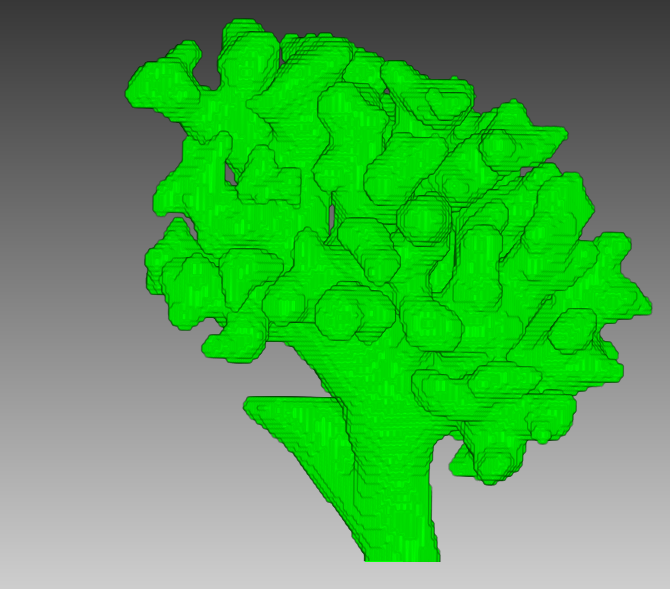
\includegraphics[width=\imagewidth]{img/skeleton/segment-crop0041}};
		\draw[|-|,thick] (25,550) -- (175,550) node[midway,above] {\unit{300}{\micro\meter}};
		\end{tikzpicture}}
		\subfloat[Overlay of \subref{fig:segment} and \subref{fig:skeleton}]{\label{fig:overlay}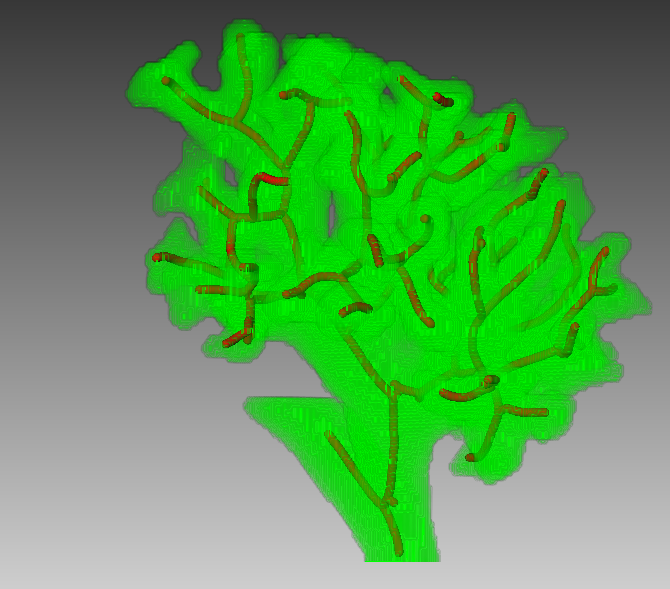
\includegraphics[width=\imsize]{img/skeleton/overlay-crop0041}}
		\subfloat[Skeleton]{\label{fig:skeleton}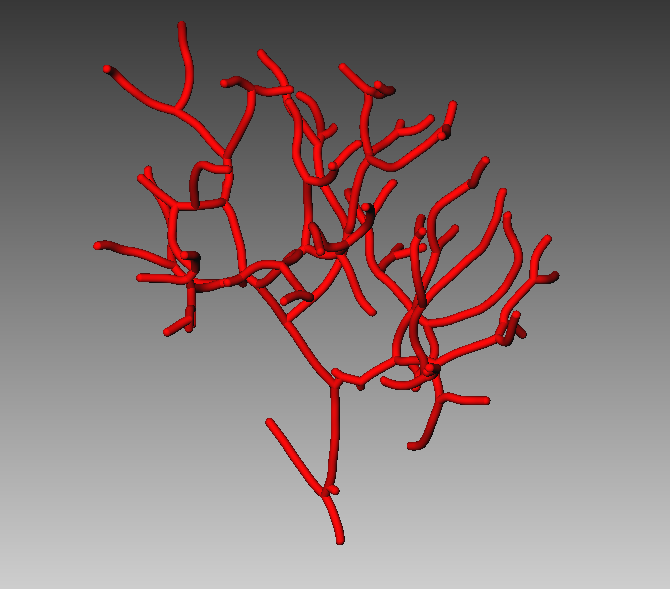
\includegraphics[width=\imsize]{img/skeleton/skel-crop0041}}
	\caption{Results of the skeletonization of the airways of a partial acinus from a Sprague Dawley rat four days after birth. An segmented acinus located at the tip of a scanned lung sample, directly underneath the pleura has been extracted from the tomographic dataset. A part of this segment has been used for the extraction of the skeleton, this part is shown in~\subref{fig:segment}. Panel \subref{fig:overlay} shows the skeleton inside the half transparent airway segment. The skeleton of the acinar airways is shown in red in panel~\subref{fig:skeleton}.}
	\todo[inline]{Correct scalebar?}
	\label{fig:skeletonization}
\end{figure}

\section{Wide field scanning}
\label{sec:wide field scanning}
Various applications depend on the availability of high resolution tomographic images of the studied sample. The available field of view (FOV) of microscopy based imaging methods like SRXTM and micro-computed tomography stations is limited through the camera and microscope optics. The FOV can only be increased if the magnification of the microscope optics is decreased, thus decreasing the available resolution. At TOMCAT, this constraint leads to the condition, that the FOV is as low as 0.72$\times$\unit{0.72}{\milli\meter} for the highest resolution (with a pixel size of 350$\times$\unit{350}{\nano\meter} and a 20-fold magnification).

The field of view can be enlarged by two different methods, by stacking multiple scans and by the so called wide field scanning, which has been developed and implemented at TOMCAT by me during the past year.

\subsection{Stacking of multiple Scans}
The FOV in the direction of the rotation axis of the sample can easily be enlarged by stacking multiple scans on top of each other. This is feasible for long and thin samples and has been implemented at TOMCAT through accurate control of the end-station setup and sample position and through calibration of the machine. A schematic drawing of this method is shown in figure~\ref{fig:stacking}.
\begin{figure}[tb]
	\centering
		%\documentclass{article}
%\usepackage[pdftex,active,tightpage]{preview}
%\usepackage{tikz}
%\usetikzlibrary{arrows,shapes,backgrounds}
%\begin{document}
%\begin{preview}
\begin{tikzpicture}[thick]%,show background grid]
	%draw axes
		%\draw[ultra thick] (-10,0) -- (10,0);
		%\draw[ultra thick] (0,-10) -- (0,10);
		%\draw[ultra thick] (0,0) circle (.125);
	% rotation axis
		\draw[->] (0,-2) ++ (-50:.75) arc (-50:300:.75 and .25);
		\draw (0,-3) node[below] {Rotation axis} -- ++(0,2);
		\draw[dotted] (0,-1) -- ++(0,2);
		\draw (0,1) -- ++(0,0.25);
		\draw[dotted] (0,1.25) -- ++(0,2);
	% position 1
		\draw (0,-1) circle (1.5 and .5);
		\fill[shade,semitransparent] (-1.5,-1) arc (-180:0:1.5 and .5) -- ++(0,2) arc (0:180:1.5 and .5) -- cycle;
		\draw (-1.5,-1) arc (-180:0:1.5 and .5) -- ++(0,2) arc (0:180:1.5 and .5) -- cycle;		
		\draw (-1.5,1) arc (-180:0:1.5 and .5);
		\draw (1.5,0) node[right] {First Position};
	% position 2
		\draw (0,1.25) circle (1.5 and .5);
		\fill[shade,semitransparent] (-1.5,1.25) arc (-180:0:1.5 and .5) -- ++(0,2) arc (0:180:1.5 and .5) -- cycle;
		\draw (-1.5,1.25) arc (-180:0:1.5 and .5) -- ++(0,2) arc (0:180:1.5 and .5) -- cycle;		
		\draw (-1.5,3.25) arc (-180:0:1.5 and .5);
		\draw (1.5,2.25) node[right] {Second Position};
	% rotation axis on top
		\draw[->] (0,3.25) -- ++(0,1.5);									
	% sample movement
		\draw[->] (-2.5,0) -- (-2.5,2) node [text width=1.75cm,midway,left] {Sample movement relative to beam and camera};	
\end{tikzpicture}
%\end{preview}
%\end{document}
	\caption{Increasing the field of view in vertical direction. feasible for long and thin samples. Two different scans are acquired and reconstructed. Thorough calibration ensures that the resulting image stacks can simply be stacked on top of each other. For illustration purposed the two positions are shown with a slight gap, in reality the sample is moved in such a fashion that the top slice of the data set obtained at the first position is adjacent to the bottom slice of the dataset obtained at the second position}
	\label{fig:stacking}
\end{figure}

\subsection{Wide Field Scanning}
\label{sec:wfs-details}
Increasing the FOV in horizontal direction of the sample is not a similarly easy task, since the obtained projection images have to be merged together to one big projection prior to be able to reconstruct the tomographic dataset of the sample.

Details in Fig~\ref{fig:wide field scan setup}, result of (different amount of subscans!) in fig~\ref{fig:wide field scan results}.
\begin{figure}[tb]
	\centering
		%\documentclass{article}
%\usepackage[pdftex,active,tightpage]{preview}
%\usepackage{tikz}
%\begin{document}
%\begin{preview}
\begin{tikzpicture}[thick]%,show background grid]
	%draw axes
		%\draw[ultra thick] (-10,0) -- (10,0);
		%\draw[ultra thick] (0,-10) -- (0,10);
		%\draw[ultra thick] (0,0) circle (.125);
	% rotation axis
		\draw[->] (0,-3) ++ (-50:.75) arc (-50:300:.75 and .25);
		\draw[] (0,-4) node[below] {Rotation axis} -- ++(0,3);
		\draw[dotted] (0,-1) -- ++(0,2);
	% position 1
		\draw (0,-1) circle (1.5 and .5);
		\fill[shade,semitransparent] (-1.5,-1) arc (-180:0:1.5 and .5) -- ++(0,2) arc (0:180:1.5 and .5) -- cycle;
		\draw (-1.5,-1) arc (-180:0:1.5 and .5) -- ++(0,2) arc (0:180:1.5 and .5) -- cycle;		
		\draw (-1.5,1) arc (-180:0:1.5 and .5);
		\draw (1.25,-1.5) node[right] {First Position};
	% position 2
		\draw (0,-1) circle (4.5 and 1.5);
		\fill[shade,semitransparent] (-4.5,-1) arc (-180:0:4.5 and 1.5) -- ++(0,2) arc (0:180:4.5 and 1.5) -- cycle;
		\draw (-4.5,-1) arc (-180:0:4.5 and 1.5) -- ++(0,2) arc (0:180:4.5 and 1.5) -- cycle;		
		\draw (-4.5,1) arc (-180:0:4.5 and 1.5);
		\draw (2.25,-2.7) node[right] {Second Position};
	% top from position 1 on top
		\draw (0,1) circle (1.5 and .5);
	% rotation axis on top
		\draw[->] (0,1) -- ++(0,2.5);									
	% sample movement
		\draw[->] (0,1) -- (3,1) node [text width=3cm,above] {Sample movement relative to beam and camera};	
\end{tikzpicture}
%\end{preview}
%\end{document}
	\caption{Increasing the field of view in horizontal direction through so called wide field scanning. Details of the scanning method are described in section~\ref{sec:wfs-details} Note that if a scan has been performed like that, we can stack multiple wide field scans on top of each other as shown in figure~\ref{fig:stacking} to additionally increase the FOV in vertical direction.}
	\label{fig:wide field scan setup}
\end{figure}

\begin{itemize}
	\item Wide Field Scanning Masterarbeit PSI
	\item Masterarbeit NDS, aber auch Projekt, dass wir verwenden k�nnen f�r Skelettierung
	\item Overlap > fig \ref{fig:merge-proj} smaller than 3$*$size(SubScan)
	\item MATLAB-Programmierung
	\item implementierung an der Beamline geplant f�r Fr�hling 2009
\end{itemize}



\renewcommand{\imsize}{.25\linewidth}
\pgfmathsetlength{\imagewidth}{\imsize} % desired displayed width of image
\pgfmathsetlength{\imagescale}{\imagewidth/512} % pixel width of image

\begin{figure}[p]
	\centering
		\subfloat[Uncorrected projection image from subscan s$_1$ with a size of 1024$\times$1024 pixels at a resolution of \unit{0.7}{\micro\meter\per pixel}.]{%
			\label{fig:s1}%
			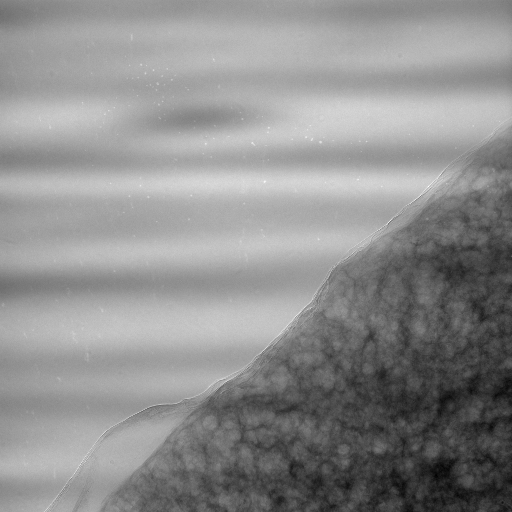
\includegraphics[width=\imsize]{img/merge/R108C10B-s1}%
			}%\
		\subfloat[Uncorrected projection image from subscan s$_2$.]{%
			\label{fig:s2}%
			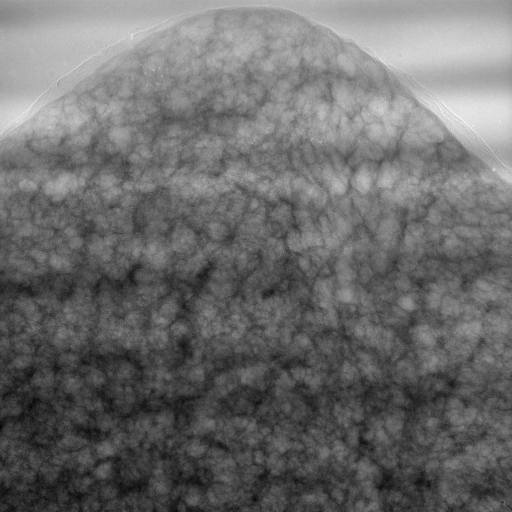
\includegraphics[width=\imsize]{img/merge/R108C10B-s2}%
			}%\
		\subfloat[Uncorrected projection image from subscan s$_3$.]{%
			\label{fig:s3}%
			\begin{tikzpicture}[x=\imagescale,y=-\imagescale]
				% place image (integer coordinates refer to pixel centers):
				\node[anchor=north west,inner sep=0pt,outer sep=0pt] at (0,0)
  					{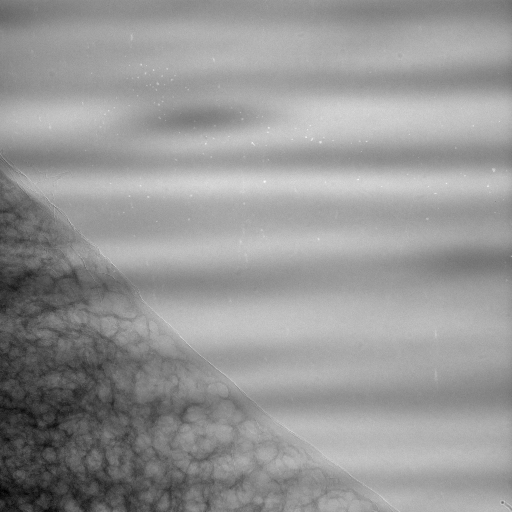
\includegraphics[width=\imagewidth]{img/merge/R108C10B-s3}};
				\draw[|-|,thick,color=white] (256-64,450) -- (512-64,450) node[midway,above] {\unit{700}{\micro\meter}};
				\end{tikzpicture}%
			}%\
		\renewcommand{\imsize}{.75\linewidth}
		\pgfmathsetlength{\imagewidth}{\imsize} % desired displayed width of image
		\pgfmathsetlength{\imagescale}{\imagewidth/1498} % pixel width of image
		\subfloat[Merged and corrected image from the three subscans shown above. The merged projections have a size of 2994$\times$1024 pixels at a resolution of \unit{0.7}{\micro\meter\per pixel}. The Subscans s$_1$--s$_3$ overlap each other by approximately 150 pixels, thus the width of the merged projection is smaller than three times the width of the subscans. 4676 projection images like the one shown here have been obtained over a sample rotation of \unit{180}{\degree} and are then reconstructed into a tomographic dataset using filtered backprojection.]{%
			\label{fig:merge-proj}%
			\begin{tikzpicture}[x=\imagescale,y=-\imagescale]
				% place image (integer coordinates refer to pixel centers):
				\node[anchor=north west,inner sep=0pt,outer sep=0pt] at (0,0)
  					{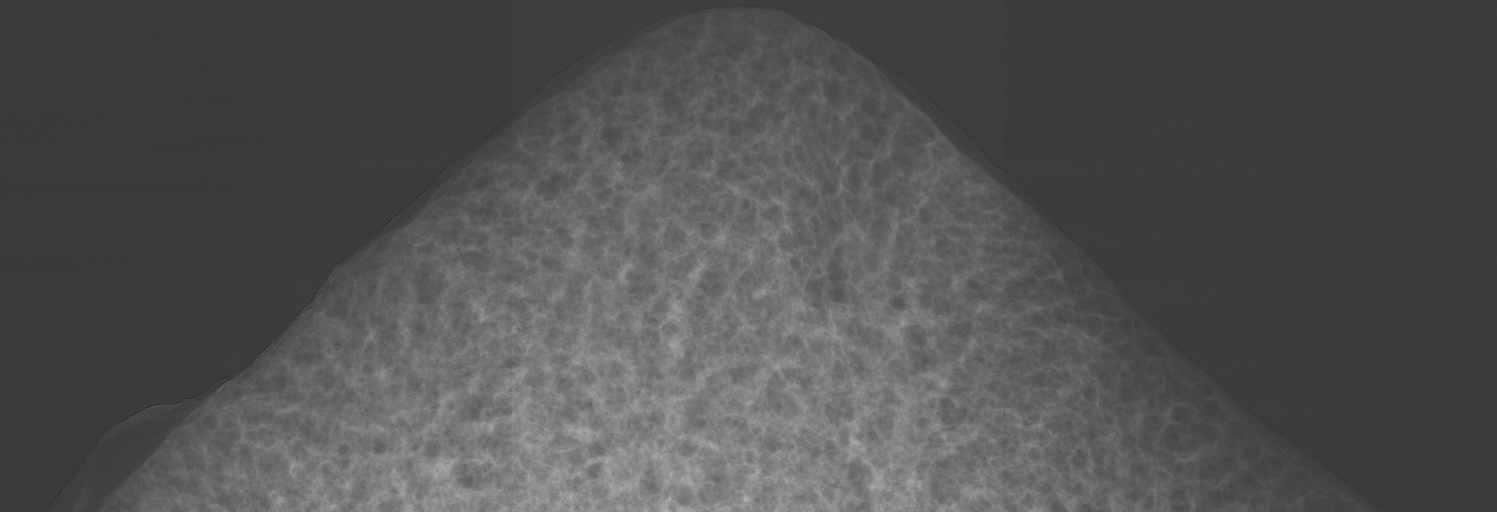
\includegraphics[width=\imagewidth]{img/merge/R108C10B-merge}};
				\draw[|-|,thick,color=white] (1240-64,450) -- (1498-64,450) node[midway,above] {\unit{700}{\micro\meter}};
			\end{tikzpicture}%
			}\\
		\pgfmathsetlength{\imagescale}{\imagewidth/1365} % pixel width of image (image has been resized from 2994*1123, so that scalebar is at the same height without calculating too much...)
		\subfloat[Cropped part of one slice of the tomographic dataset reconstructed from the merged projections, where one is shown in subfigure~\subref{fig:merge-proj}. The halo directly around the lung tissue arises from the paraffin where the sample is embedded in. The inset on the upper left corner shows an overview over the full slice. The bright circular shape inscribed in the square arises from the filtered backprojection, the chosen reconstruction method. The size of the cropped image is 2994$\times$1123 pixels.]{%
			\label{fig:merge-rec}%
			\begin{tikzpicture}[x=\imagescale,y=-\imagescale]
				% place image (integer coordinates refer to pixel centers):
				\node[anchor=north west,inner sep=0pt,outer sep=0pt] at (0,0)
  					{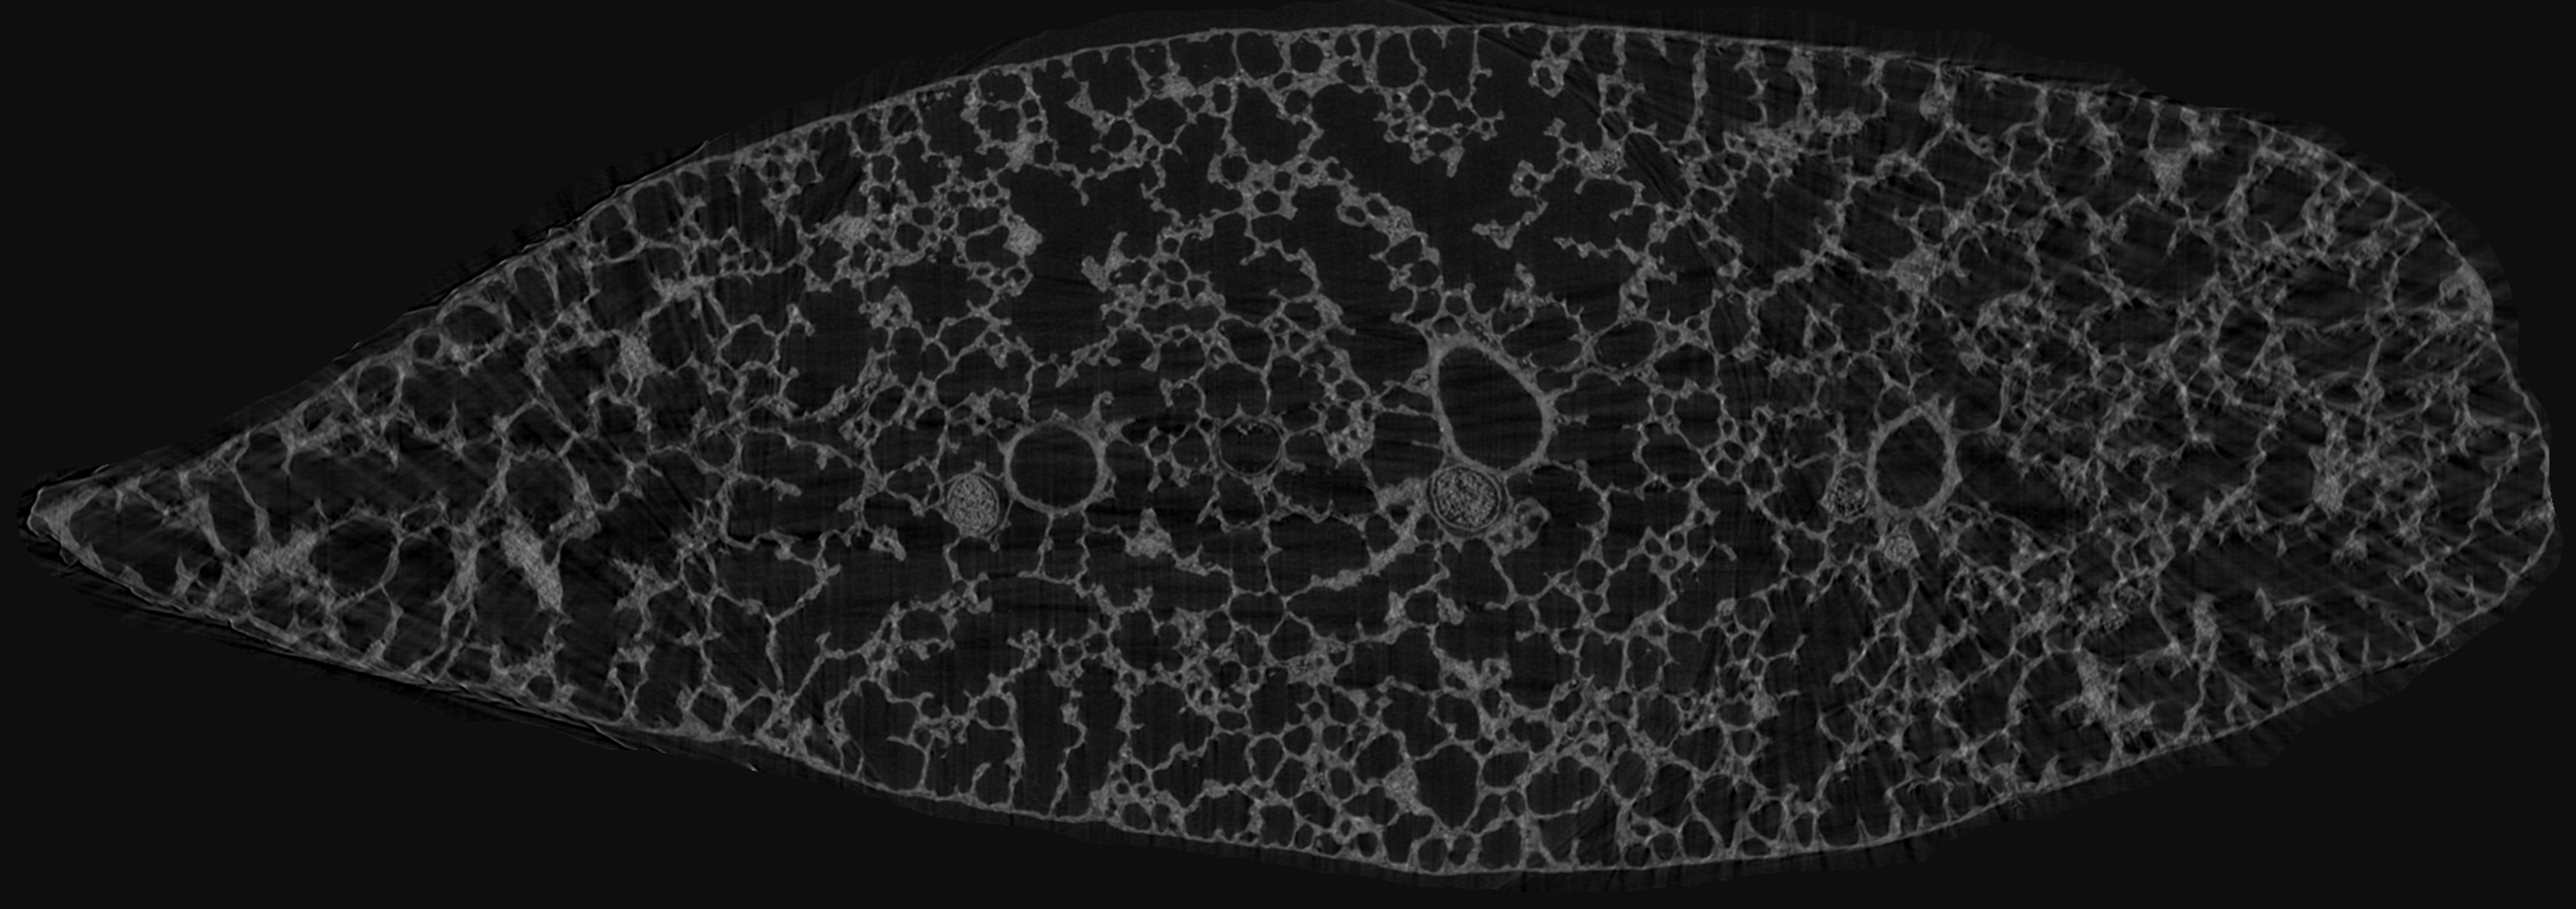
\includegraphics[width=\imagewidth]{img/merge/R108C10B-merge1016-crop}};
  				\newcommand{\size}{.2\imagewidth}
  				\node[anchor=north west,inner sep=0pt,outer sep=0pt] at (0,0)
  					{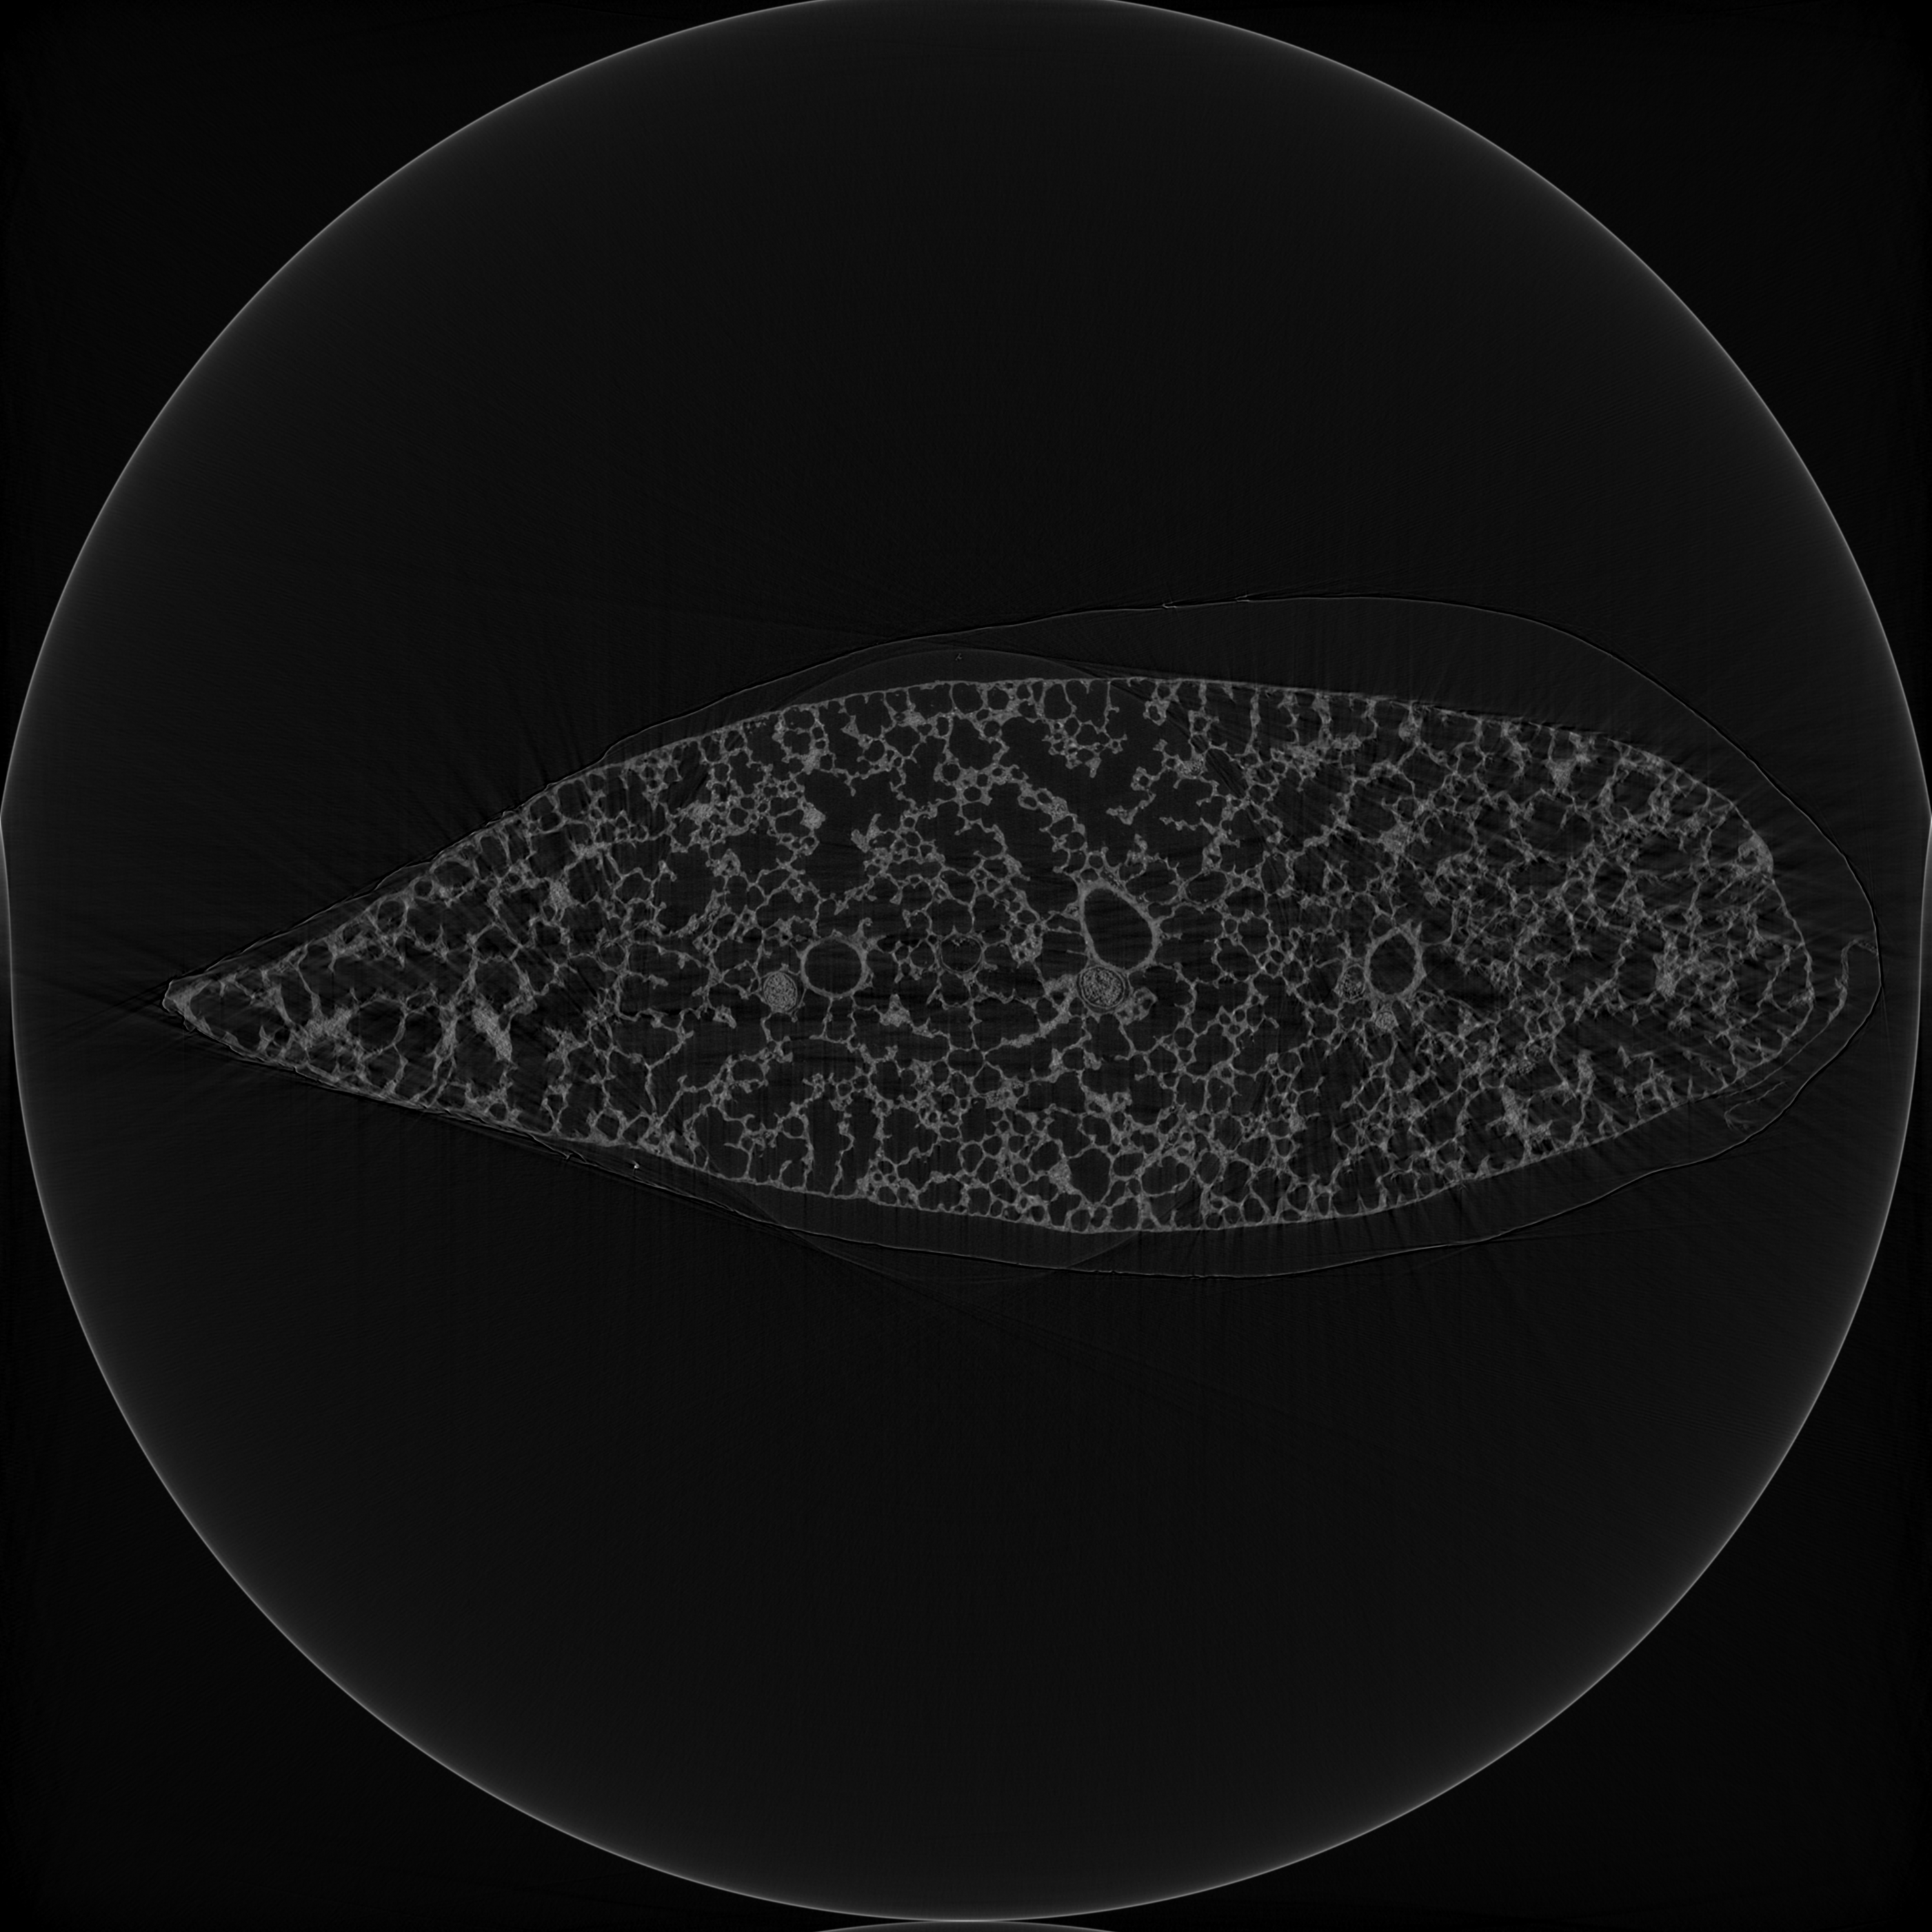
\includegraphics[width=\size]{img/merge/R108C10B-merge1016}};
  				\draw[white] (\size,0) -- (\size,-\size) -- (0,-\size);
				\draw[|-|,thick,color=white] (1109-64,450) -- (1365-64,450) node[midway,above] {\unit{700}{\micro\meter}};
			\end{tikzpicture}%
			}\\
	\caption{Wide Field Scan Results for a rat lung sample 10 days after birth, showing the distal tip of the right under lung lobe.}
	\label{fig:wide field scan results}
	\todo[inline]{distal tip of RUL: true? > askJohannes}
	\todo[inline]{Correct scalebar? Messung-2008b.xls}

\end{figure}



\section{Outlook}
\begin{itemize}
	\item Skelettierung, Segmente anzeichnen, damit Statistik gemacht werden kann
	\item Wide Field scanning perfektionieren, Implementierung an der Beamline
\end{itemize}

\section{Publications}
\label{sec:publications}
Our group has been working on a publication to show the comparability of measurements obtained with SRXTM with classical morphological experiments. The paper~\cite{Tsuda2008} has been published this summer, I am one of the co-authors and have provided three figures, and substantial parts of the text.

As described in section~\ref{sec:multimodal imaging}, the multimodal imaging method has been successfully established at our institute. I have presented this method as a poster at two conferences~\cite{Haberthuer2008,Haberthuer2008b} and submitted a proceeding to the Journal of Physics after the second conference~\cite{Haberthuer2009}.

The preliminary results of my skeletonization method have been presented at a talk at the 'Tag der Anatomie'~\cite{Haberthuer2008a}, it is planned that --- now that the method is applicable to our samples --- we prepare a publication of this method.

The wide field scanning method has been thoroughly described in my master thesis of the MAS in Medical Physics~\cite{Haberthuer2008c} and presented in front of the other master students~\cite{Haberthuer2008d}. I am now in the process of writing a publication now that additional experiments to prove the simulations and predictions have been carried out.

\bibliographystyle{unsrtnat}
\bibliography{../../references}
\end{document}